\documentclass{ctexart}
\usepackage[utf8]{inputenc}
\usepackage{graphicx}
\usepackage{tikz}
\usetikzlibrary{shapes,arrows}


\title{作业3: AVL Tree}
\author{陈科辉 Keiver Pabula}
\date{28 Octobe,2022}
\begin{document}
\maketitle

作业3:AVL Tree
\section{设计思路}
题目要求我们制作一个平衡书,输入元素k1,k2为上下限遍历树中所有在这之间的元素,并为他们排序输出,并且还需要记录其时间来观察它的复杂性。因此我先拿了头文件AVLTree.h并为其制作Printelement函数,其中这个程序符合了(k1为下限,k2为上限):
若节点为空,什么也不做;其实就是在排除k1>k2的情况;
在k1<k<k2的情况下,则将元素按顺序排列,并将他们全部打印出来。

  因为是要记录时间,所以使用时间函数。并且因为要多次实验,所以我将主函数设计为多次不同元素的排序。元素每次增加100,且k1和k2恒定,所以元素增加的情况下,范围不变进行排序。
\section{理论分析}
  首先树有两类:1类在要求内,第2类不再要求内。因为是AVLTree所有的点应该最多高度只差1.设在k1到k2之间有K个元素,所以出输出K次,所以运行O(K)次;除了输出的点还有那些不再k1到k2的点需要跟着进行判断他是否在里面,而数的高度为O(logN),所以要执行O(logN)次,所以总共为O(K + logN).

  \section{数值结果}
  通过结果可以发现符合理论分析的结果,复杂度为O(K+logN)
\begin{center}
  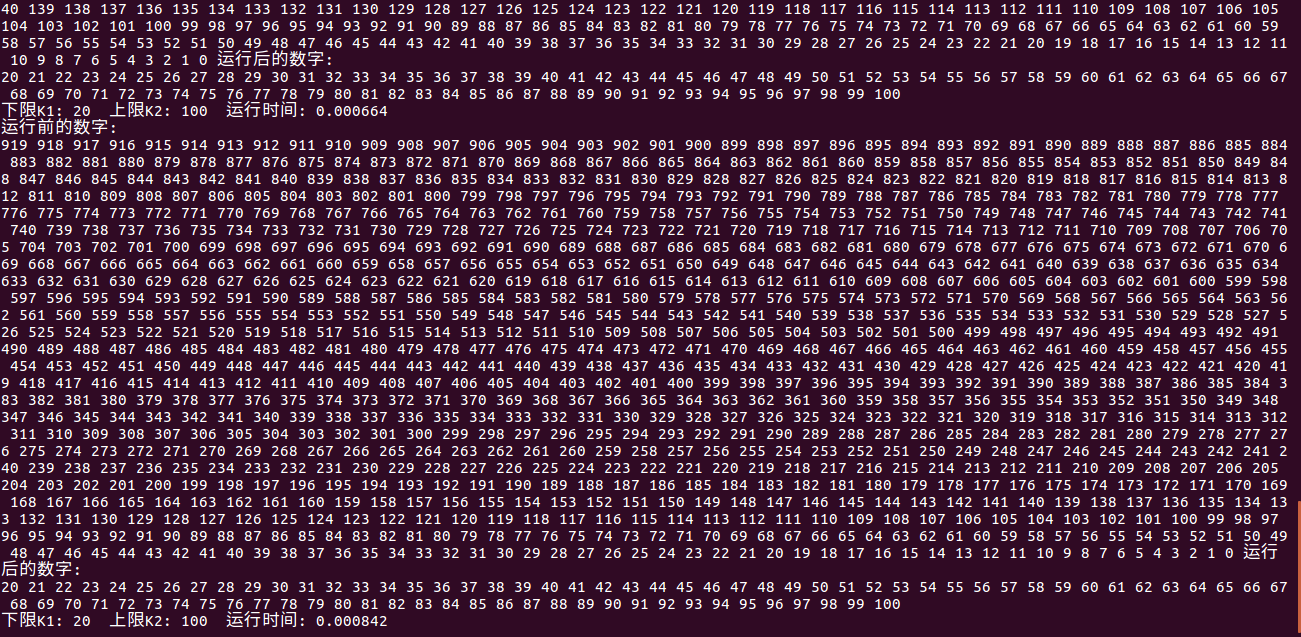
\includegraphics[scale=0.25]{1.png}
  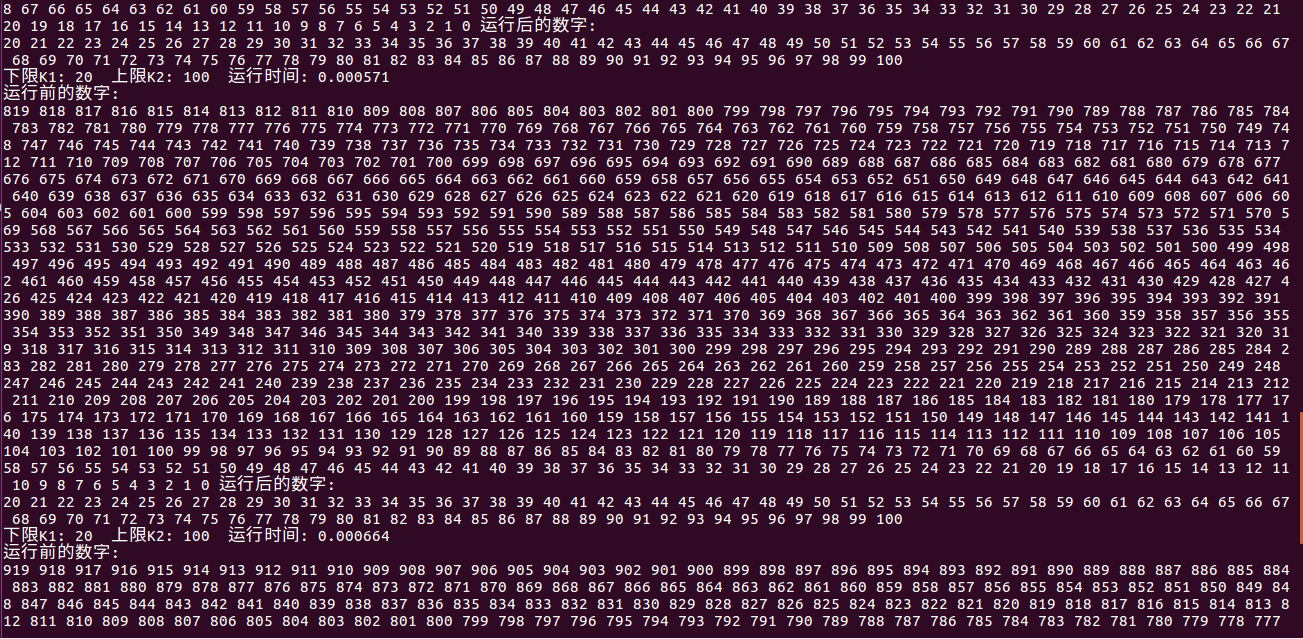
\includegraphics[scale=0.25]{2.png}
\end{center}
\begin{center}
  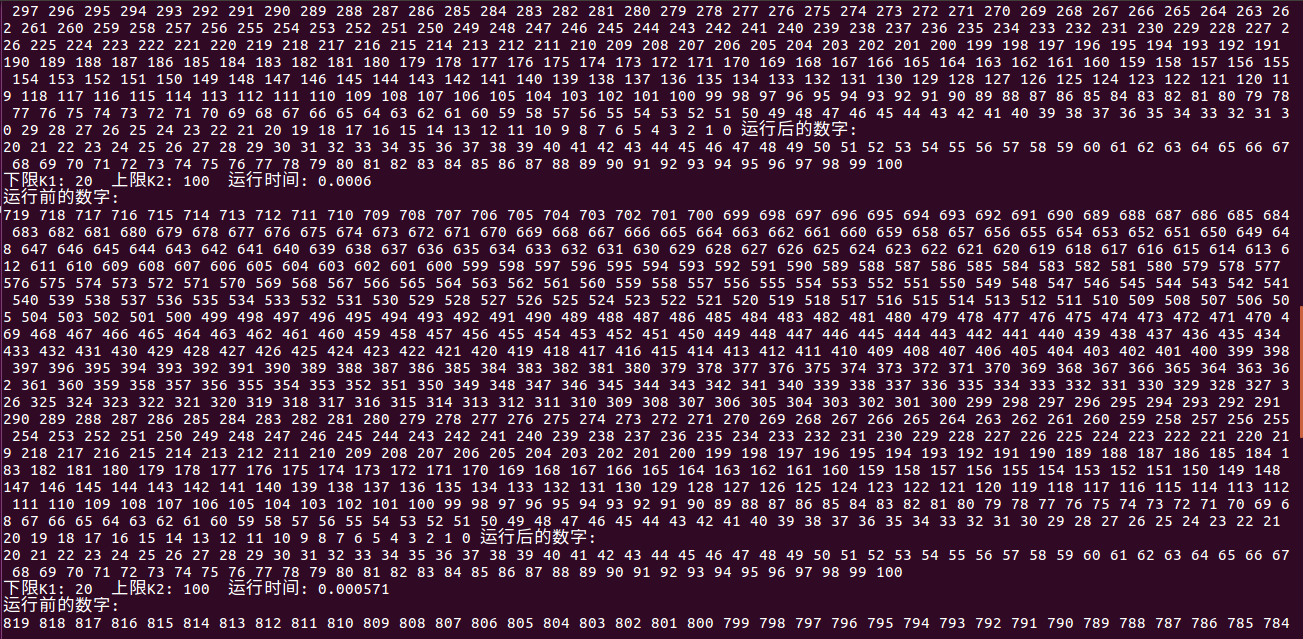
\includegraphics[scale=0.25]{3.png}
  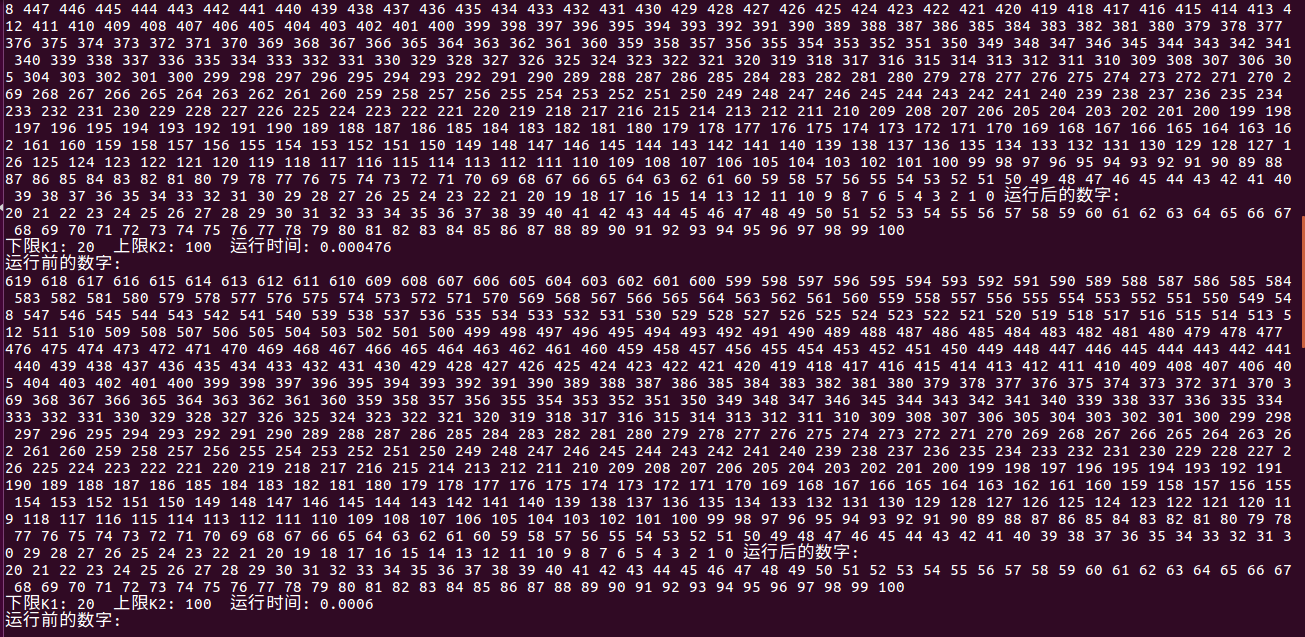
\includegraphics[scale=0.25]{4.png}
\end{center}
\begin{center}
  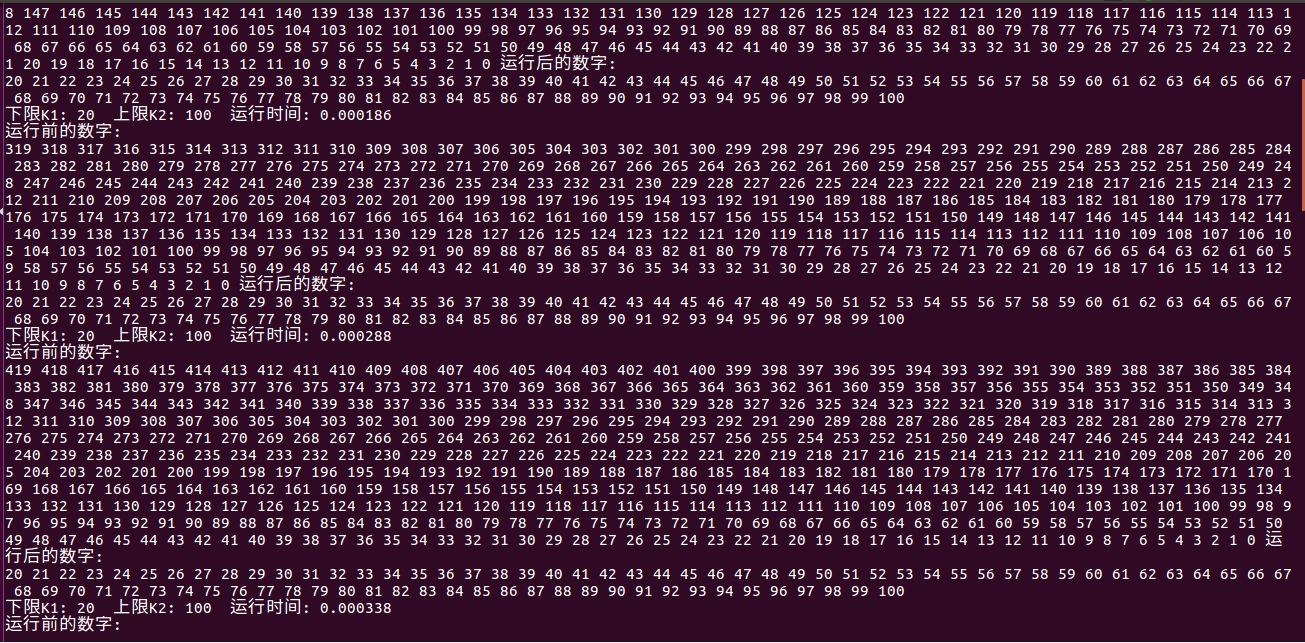
\includegraphics[scale=0.25]{5.png}
  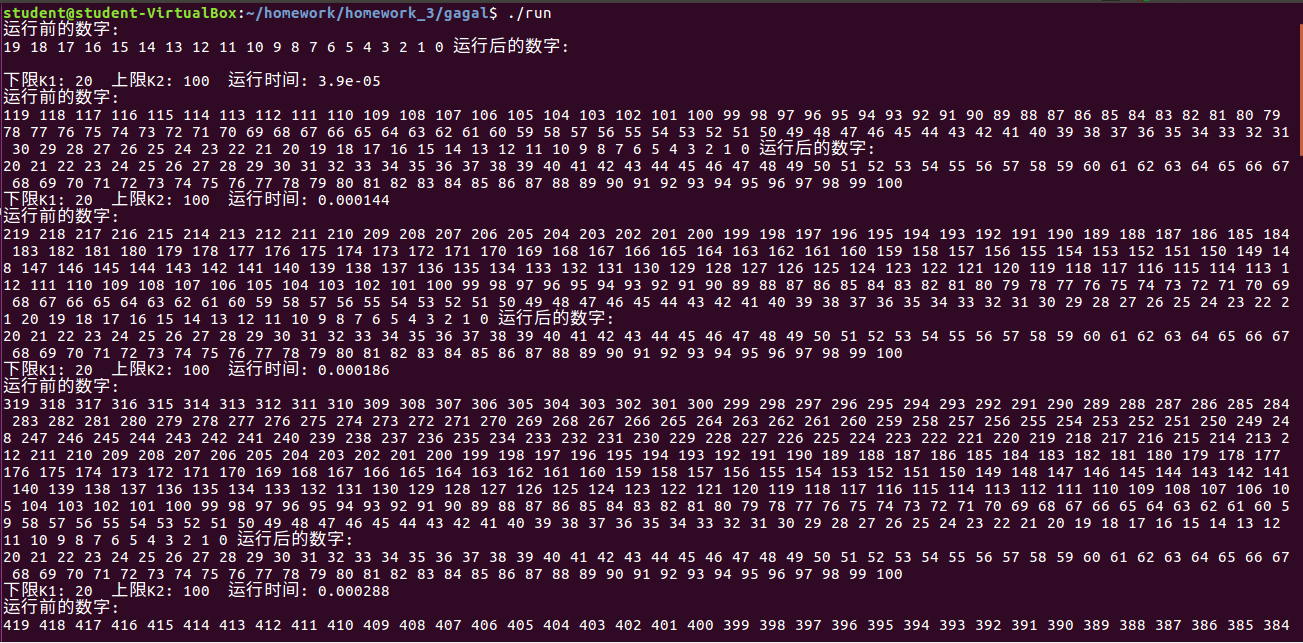
\includegraphics[scale=0.25]{6.png}
\end{center}

\end{document}
